\chapter{Interoperability}
Interoperability is the ability of making systems and organizations to work together.
There is many uses for the term, I will here use it in terms of software and medical industry.
Interoperability can be defined as:
\begin{quote}
The capability to communicate, execute programs, or transfer data among various functional units in a manner that requires the user to have little or no knowledge of the unique characteristics of those units.\cite{12}
\end{quote}
\begin{itemize}
\item Why is it a problem?
\item How does it become a problem?
\item Now that we are here, are there any solutions. 
\item When the syntax is right, but the semantics isnt.
\item When the semantics is right, but the syntax isnt.
\item Silos!!!
\item Få med fler kilder
\item verktøy og metoder
\end{itemize}
\section{An overview}
\section{Ways to achieve interoperability}
\section{Experiences}
I would like to re-present some data collected and analyzed by a group of scientists (See bibliography \cite{11}).
\begin{figure}
\centering
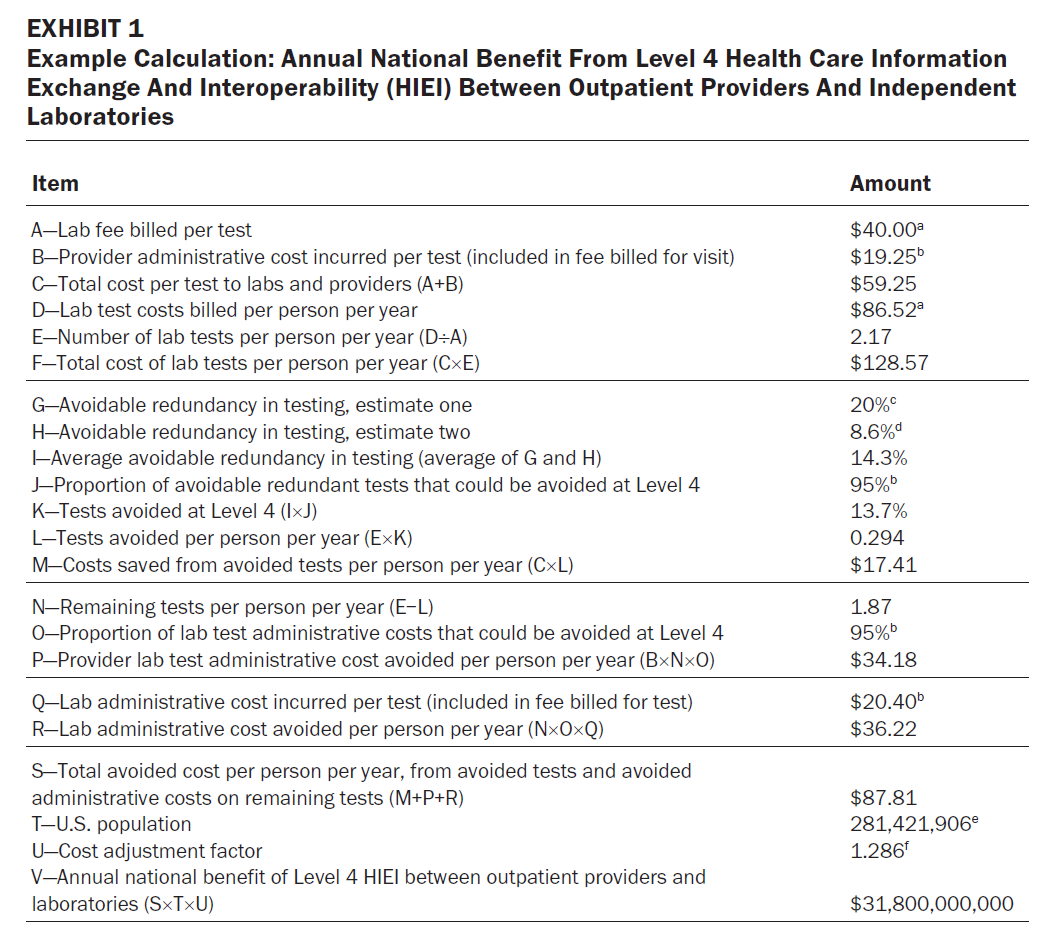
\includegraphics[width=12cm]{litterature/images/exhibit1}
\caption{Exhibit 1}
\label{fig:exhibit_1}
\end{figure}
\begin{figure}
\centering
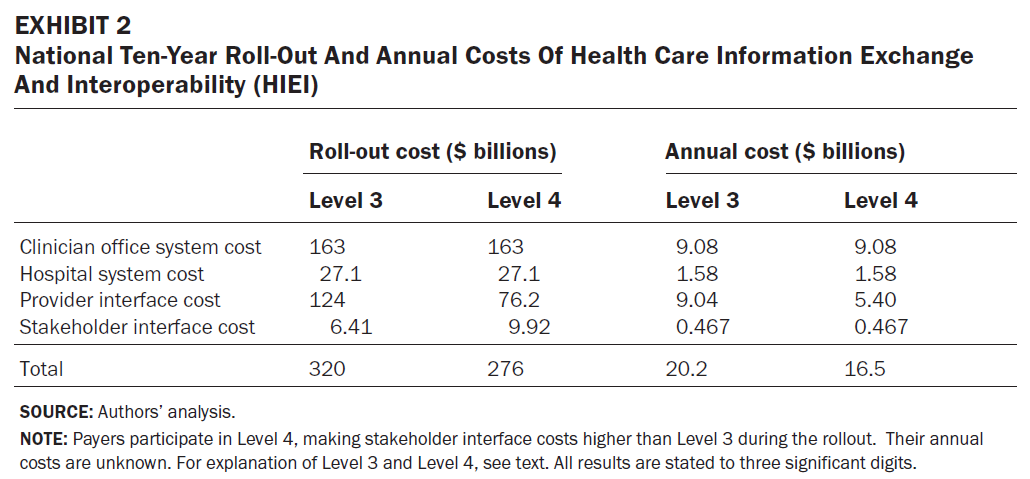
\includegraphics[width=12cm]{litterature/images/exhibit2}
\caption{Exhibit 2}
\label{fig:exhibit_2}
\end{figure}
These numbers are based on upgrading the health information system in USA. As you can see from \ref{fig:exhibit_1}, there is alot of costs that could be saved in terms of financial gain.
They have used an analytical framwork for categorizing the amount of human involvement required, the sophistication of IT, and the level of standardization. The categorization is made up by four levels.
\begin{description}
\item[Level 1]Nonelectronic data—no use of IT to share information (examples: mail, telephone).
\item[Level 2]Machinetransportable data—transmission of nonstandardized information via basic IT; information within the document cannot be electronically manipulated (examples: fax or personal computer [PC]–based exchange of scanned documents, pictures, or portable document format [PDF] files).
\item[Level 3]Machine-organizable data—transmission of structured messages containing nonstandardized data; requires interfaces that can translate incoming data from the sending organization’s vocabulary to the receiving organization’s vocabulary; usually results in imperfect translations because of vocabularies’ incompatible levels of detail (examples: e-mail of free text, or PC-based exchange of files in incompatible/proprietary file formats, HL-7 messages).
\item[Level 4]Machine-interpretable data—transmission of structured messages containing standardized and coded data; idealized state in which all systems exchange information using the same formats and vocabularies (examples: automated exchange of coded results from an external lab into a provider’s EMR, automated exchange of a patient’s “problem list”).
\end{description}
In addition, interoperability between health care instances would reduce errors, increase efficiency and open up for even more interoperability cross fields of profession. Any government would easily see the future benfits of investing in such a project.
 